\chapter{Spécification des besoins}

\begin{spacing}{1.2}
\minitoc
\thispagestyle{MyStyle}
\end{spacing}
\newpage

\section*{INTRODUCTION}

\noindent Dans ce chapitre, nous analysons les besoins de l'application « Prévention Plus » en identifiant les acteurs, les besoins fonctionnels et non fonctionnels. Ensuite, nous présentons une analyse globale avec les diagrammes des classes et des cas d'utilisation, et enfin, nous détaillons la planification des sprints pour le développement du projet.

\section{Spécification de besoins :}

\subsection{Acteurs :}

\noindent Un acteur est une entité externe, humaine ou technique, qui interagit directement avec le système à développer.

\noindent\textbf{Super Admin} : Cet acteur supervise l'ensemble du système, gérant les utilisateurs, les entreprises, les rôles, les abonnements, la taxonomie, et les notifications.

\noindent\textbf{Admin} : Cet acteur gère les utilisateurs de son entreprise, les revues de direction, les paramètres d'entreprise, tout en accédant aux fonctionnalités d'audit et de conformité.

\noindent\textbf{Auditeur} : Cet acteur participe aux revues de direction et complète les plans d'action au sein de son entreprise, avec des droits d'accès limités aux fonctionnalités essentielles.

\subsection{Besoins fonctionnels :}

\noindent Les besoins fonctionnels sont organisés selon les acteurs à qui ils sont destinés.

\noindent\textbf{Espace de l'acteur Super Admin :}

\noindent Cet espace est uniquement accessible par le super administrateur. Ses fonctionnalités sont :

\begin{itemize}
  \item Authentification : Le super admin doit s'identifier à l'aide d'un email et d'un mot de passe pour accéder à son espace.
  \item Gérer les requêtes d'inscription : accepter ou rejeter les demandes d'inscription des entreprises.
  \item Gérer les entreprises : consulter et supprimer les entreprises du système.
  \item Gérer les utilisateurs : consulter et supprimer tous les utilisateurs du système.
  \item Gérer les notifications : consulter les notifications du système.
  \item Gérer les textes : consulter, supprimer et filtrer les textes réglementaires.
  \item Consulter les statistiques : accéder aux données analytiques globales du système.
  \item Gérer les plans d'abonnement : créer, consulter, modifier, supprimer et désactiver les plans d'abonnement.
  \item Consulter l'historique : accéder à l'historique complet des utilisateurs du site.
  \item Gérer son profil : consulter et modifier ses informations personnelles.
  \item Gérer la taxonomie : créer, consulter et supprimer les éléments de classification du système.
\end{itemize}

\noindent\textbf{Espace de l'acteur Admin :}

\noindent Cet espace est accessible par les administrateurs d'entreprise. Les fonctionnalités qui leur sont associées sont :

\begin{itemize}
  \item Authentification : l'admin doit s'identifier à l'aide d'un email et d'un mot de passe pour accéder à son espace.
  \item S'inscrire : créer un compte administrateur et enregistrer son entreprise simultanément.
  \item Gérer les notifications : consulter les notifications relatives à son activité.
  \item Gérer les textes : créer, consulter, modifier et supprimer les textes réglementaires de son entreprise.
  \item Consulter les statistiques : accéder aux tableaux de bord et indicateurs de conformité de son entreprise.
  \item Gérer son profil : consulter et modifier ses informations personnelles.
  \item Gérer les utilisateurs de son entreprise : créer, consulter, modifier et supprimer les comptes utilisateurs de son organisation.
  \item Gérer les revues de direction : créer, consulter, modifier et supprimer les revues de direction.
  \item Participer aux revues de direction : consulter, créer, modifier et supprimer les éléments des revues, avec la possibilité de marquer le statut comme complété ou annulé.
  \item Gérer les paramètres de son entreprise : consulter et modifier la configuration de son organisation.
  \item Souscrire à un plan d'abonnement : consulter les plans disponibles et s'abonner.
  \item Consulter l'évaluation de la conformité : accéder aux évaluations de conformité réglementaire.
  \item Gérer les plans d'action : créer, consulter, modifier et supprimer les plans d'action.
  \item Consulter l'historique : accéder à l'historique des utilisateurs de son entreprise.
\end{itemize}

\noindent\textbf{Espace de l'acteur Auditeur :}

\noindent Cet espace est accessible par les auditeurs. Les fonctionnalités qui leur sont associées sont :

\begin{itemize}
  \item Authentification : l'auditeur doit s'identifier à l'aide d'un email et d'un mot de passe pour accéder à son espace.
  \item Gérer les notifications : consulter les notifications relatives à son activité.
  \item Gérer son profil : consulter et modifier ses informations personnelles.
  \item Participer aux revues de direction : consulter, créer, modifier et supprimer les éléments des revues.
  \item Consulter son historique : accéder à l'historique de ses actions.
  \item Compléter les plans d'action : consulter et modifier les plans d'action qui lui sont assignés avec des suggestions IA pour améliorer leur efficacité.
\end{itemize}


\subsection{Besoins non fonctionnels :}

\noindent \textbf{Sécurité} : L'application doit protéger les données contre les accès non autorisés, en utilisant l'authentification par e-mail unique et des protocoles sécurisés pour les connexions et la gestion des données sensibles.

\noindent\textbf{Responsivité} : L'interface doit s'adapter automatiquement aux différents appareils pour garantir une expérience utilisateur fluide, conformément aux principes du Responsive Web Design.

\noindent\textbf{Performance} : L'application doit permettre une navigation rapide et un accès en temps réel aux statistiques et aux tableaux de bord, même avec un grand volume de données réglementaires.

\section{Backlog}

\begin{longtable}{|>{\raggedright\arraybackslash}p{0.5cm}|>{\raggedright\arraybackslash}p{3cm}|>{\raggedright\arraybackslash}p{8cm}|>{\raggedright\arraybackslash}p{2cm}|}
\caption{Backlog produit}\label{tab:user_stories}\\
\hline
ID & Thème & User Stories & Priorité \\
\hline
\endfirsthead
\multicolumn{4}{c}{\tablename\ \thetable\ -- suite} \\
\hline
ID & Thème & User Stories & Priorité \\
\hline
\endhead
1 & Authentification & En tant que Super Admin, Admin ou Auditeur, je veux m'authentifier avec une adresse e-mail unique pour accéder à mes fonctionnalités. & Élevée \\
\hline
2 & Inscription & En tant qu'Admin, je veux m'inscrire et créer le compte de mon entreprise simultanément pour accéder au système. & Élevée \\
\hline
3 & Gérer les requêtes d'inscription & En tant que Super Admin, je veux accepter ou rejeter les demandes d'inscription pour contrôler l'accès au système. & Élevée \\
\hline
4 & Gérer les profils & En tant qu'utilisateur, je veux consulter mon profil pour accéder à mes informations personnelles. & Moyenne \\
\cline{3-4}
& & En tant qu'utilisateur, je veux modifier mon profil pour mettre à jour mes informations personnelles. & Moyenne \\
\hline
5 & Gérer les notifications & En tant qu'utilisateur, je veux consulter mes notifications pour rester informé des activités du système. & Faible \\
\hline
6 & Gérer les textes & En tant qu'Admin, je veux créer des textes réglementaires pour maintenir la conformité de mon entreprise. & Élevée \\
\cline{3-4}
& & En tant qu'Admin, je veux consulter les textes réglementaires de mon entreprise. & Élevée \\
\cline{3-4}
& & En tant qu'Admin, je veux modifier les textes réglementaires de mon entreprise. & Moyenne \\
\cline{3-4}
& & En tant qu'Admin, je veux supprimer les textes réglementaires de mon entreprise. & Moyenne \\
\cline{3-4}
& & En tant que Super Admin, je veux consulter tous les textes réglementaires du système. & Moyenne \\
\cline{3-4}
& & En tant que Super Admin, je veux supprimer et filtrer les textes réglementaires pour superviser le contenu. & Moyenne \\
\hline
7 & Consulter les statistiques & En tant qu'utilisateur, je veux consulter les statistiques appropriées à mon rôle pour analyser les performances et la conformité. & Faible \\
\hline
8 & Gérer les utilisateurs & En tant qu'Admin, je veux créer des utilisateurs dans mon entreprise pour organiser mon équipe. & Élevée \\
\cline{3-4}
& & En tant qu'Admin, je veux consulter les utilisateurs de mon entreprise. & Élevée \\
\cline{3-4}
& & En tant qu'Admin, je veux modifier les utilisateurs de mon entreprise. & Moyenne \\
\cline{3-4}
& & En tant qu'Admin, je veux supprimer les utilisateurs de mon entreprise. & Moyenne \\
\cline{3-4}
& & En tant que Super Admin, je veux consulter tous les utilisateurs du système. & Moyenne \\
\cline{3-4}
& & En tant que Super Admin, je veux supprimer les utilisateurs pour administrer le système. & Moyenne \\
\hline
9 & Gérer les entreprises & En tant que Super Admin, je veux consulter toutes les entreprises pour administrer la plateforme. & Moyenne \\
\cline{3-4}
& & En tant que Super Admin, je veux supprimer les entreprises pour administrer la plateforme. & Moyenne \\
\hline
10 & Gérer les revues de direction & En tant qu'Admin, je veux créer des revues de direction pour organiser les évaluations. & Moyenne \\
\cline{3-4}
& & En tant qu'Admin, je veux consulter les revues de direction de mon entreprise. & Moyenne \\
\cline{3-4}
& & En tant qu'Admin, je veux modifier les revues de direction de mon entreprise. & Moyenne \\
\cline{3-4}
& & En tant qu'Admin, je veux supprimer les revues de direction de mon entreprise. & Moyenne \\
\hline
11 & Participer aux revues de direction & En tant qu'Admin, je veux participer aux revues et marquer leur statut comme complété ou annulé pour gérer le processus d'évaluation. & Moyenne \\
\cline{3-4}
& & En tant qu'Auditeur, je veux participer aux revues en consultant, créant, modifiant et supprimant les éléments pour contribuer au processus d'évaluation. & Moyenne \\
\hline
12 & Gérer les paramètres d'entreprise & En tant qu'Admin, je veux consulter les paramètres de mon entreprise pour visualiser la configuration. & Moyenne \\
\cline{3-4}
& & En tant qu'Admin, je veux modifier les paramètres de mon entreprise pour personnaliser la configuration. & Moyenne \\
\hline
13 & Souscrire aux abonnements & En tant qu'Admin, je veux consulter les plans d'abonnement disponibles pour évaluer les options. & Élevée \\
\cline{3-4}
& & En tant qu'Admin, je veux souscrire à un plan d'abonnement pour accéder aux fonctionnalités premium. & Élevée \\
\hline
14 & Gérer les plans d'abonnement & En tant que Super Admin, je veux créer des plans d'abonnement pour configurer les offres. & Moyenne \\
\cline{3-4}
& & En tant que Super Admin, je veux modifier des plans d'abonnement pour ajuster les offres. & Moyenne \\
\cline{3-4}
& & En tant que Super Admin, je veux supprimer des plans d'abonnement pour gérer les offres. & Moyenne \\
\cline{3-4}
& & En tant que Super Admin, je veux désactiver des plans d'abonnement pour contrôler leur disponibilité. & Moyenne \\
\cline{3-4}
& & En tant que Super Admin, je veux consulter les plans d'abonnement pour superviser les offres. & Moyenne \\
\hline
15 & Consulter l'évaluation de conformité & En tant qu'Admin, je veux consulter l'évaluation de la conformité pour surveiller le respect des normes. & Élevée \\
\hline
16 & Gérer les plans d’action & En tant qu'Admin, je veux créer des plans d'action pour gérer les non-conformités. & Élevée \\
\cline{3-4}
& & En tant qu'Admin, je veux consulter les plans d'action de mon entreprise. & Élevée \\
\cline{3-4}
& & En tant qu'Admin, je veux modifier les plans d'action de mon entreprise. & Moyenne \\
\cline{3-4}
& & En tant qu'Admin, je veux supprimer les plans d'action de mon entreprise. & Moyenne \\
\cline{3-4}
& & En tant qu'Auditeur, je veux consulter les plans d'action qui me sont assignés. & Moyenne \\
\cline{3-4}
& & En tant qu'Auditeur, je veux modifier les plans d'action qui me sont assignés pour contribuer à leur réalisation. & Moyenne \\
\cline{3-4}
& & En tant qu'Auditeur, je veux recevoir des conseils IA pour optimiser la réalisation des plans d'action qui me sont assignés. & Faible \\
\hline
17 & Consulter l'historique & En tant que Super Admin, je veux consulter l'historique complet des utilisateurs du site pour assurer la supervision. & Moyenne \\
\cline{3-4}
& & En tant qu'Admin, je veux consulter l'historique des utilisateurs de mon entreprise pour assurer la traçabilité. & Moyenne \\
\cline{3-4}
& & En tant qu'Auditeur, je veux consulter mon historique pour suivre mes actions. & Moyenne \\
\hline
18 & Gérer la taxonomie & En tant que Super Admin, je veux créer des éléments de taxonomie pour organiser la classification du système. & Élevée \\
\cline{3-4}
& & En tant que Super Admin, je veux consulter la taxonomie pour superviser la classification. & Élevée \\
\cline{3-4}
& & En tant que Super Admin, je veux supprimer des éléments de taxonomie pour maintenir l'organisation du système. & Moyenne \\
\hline
\end{longtable}

\section{Analyse globale :}

\noindent Nous utilisons le langage UML pour modéliser les fonctionnalités décrites dans le tableau des user stories, afin de représenter graphiquement les interactions et la structure du système.

\subsection{Diagramme de cas d'utilisation global :}

\noindent Le diagramme de cas d'utilisation global en UML illustre les interactions entre les acteurs et le système, définissant les exigences fonctionnelles de « Prévention Plus ».

\begin{figure}[H]
    \centering
    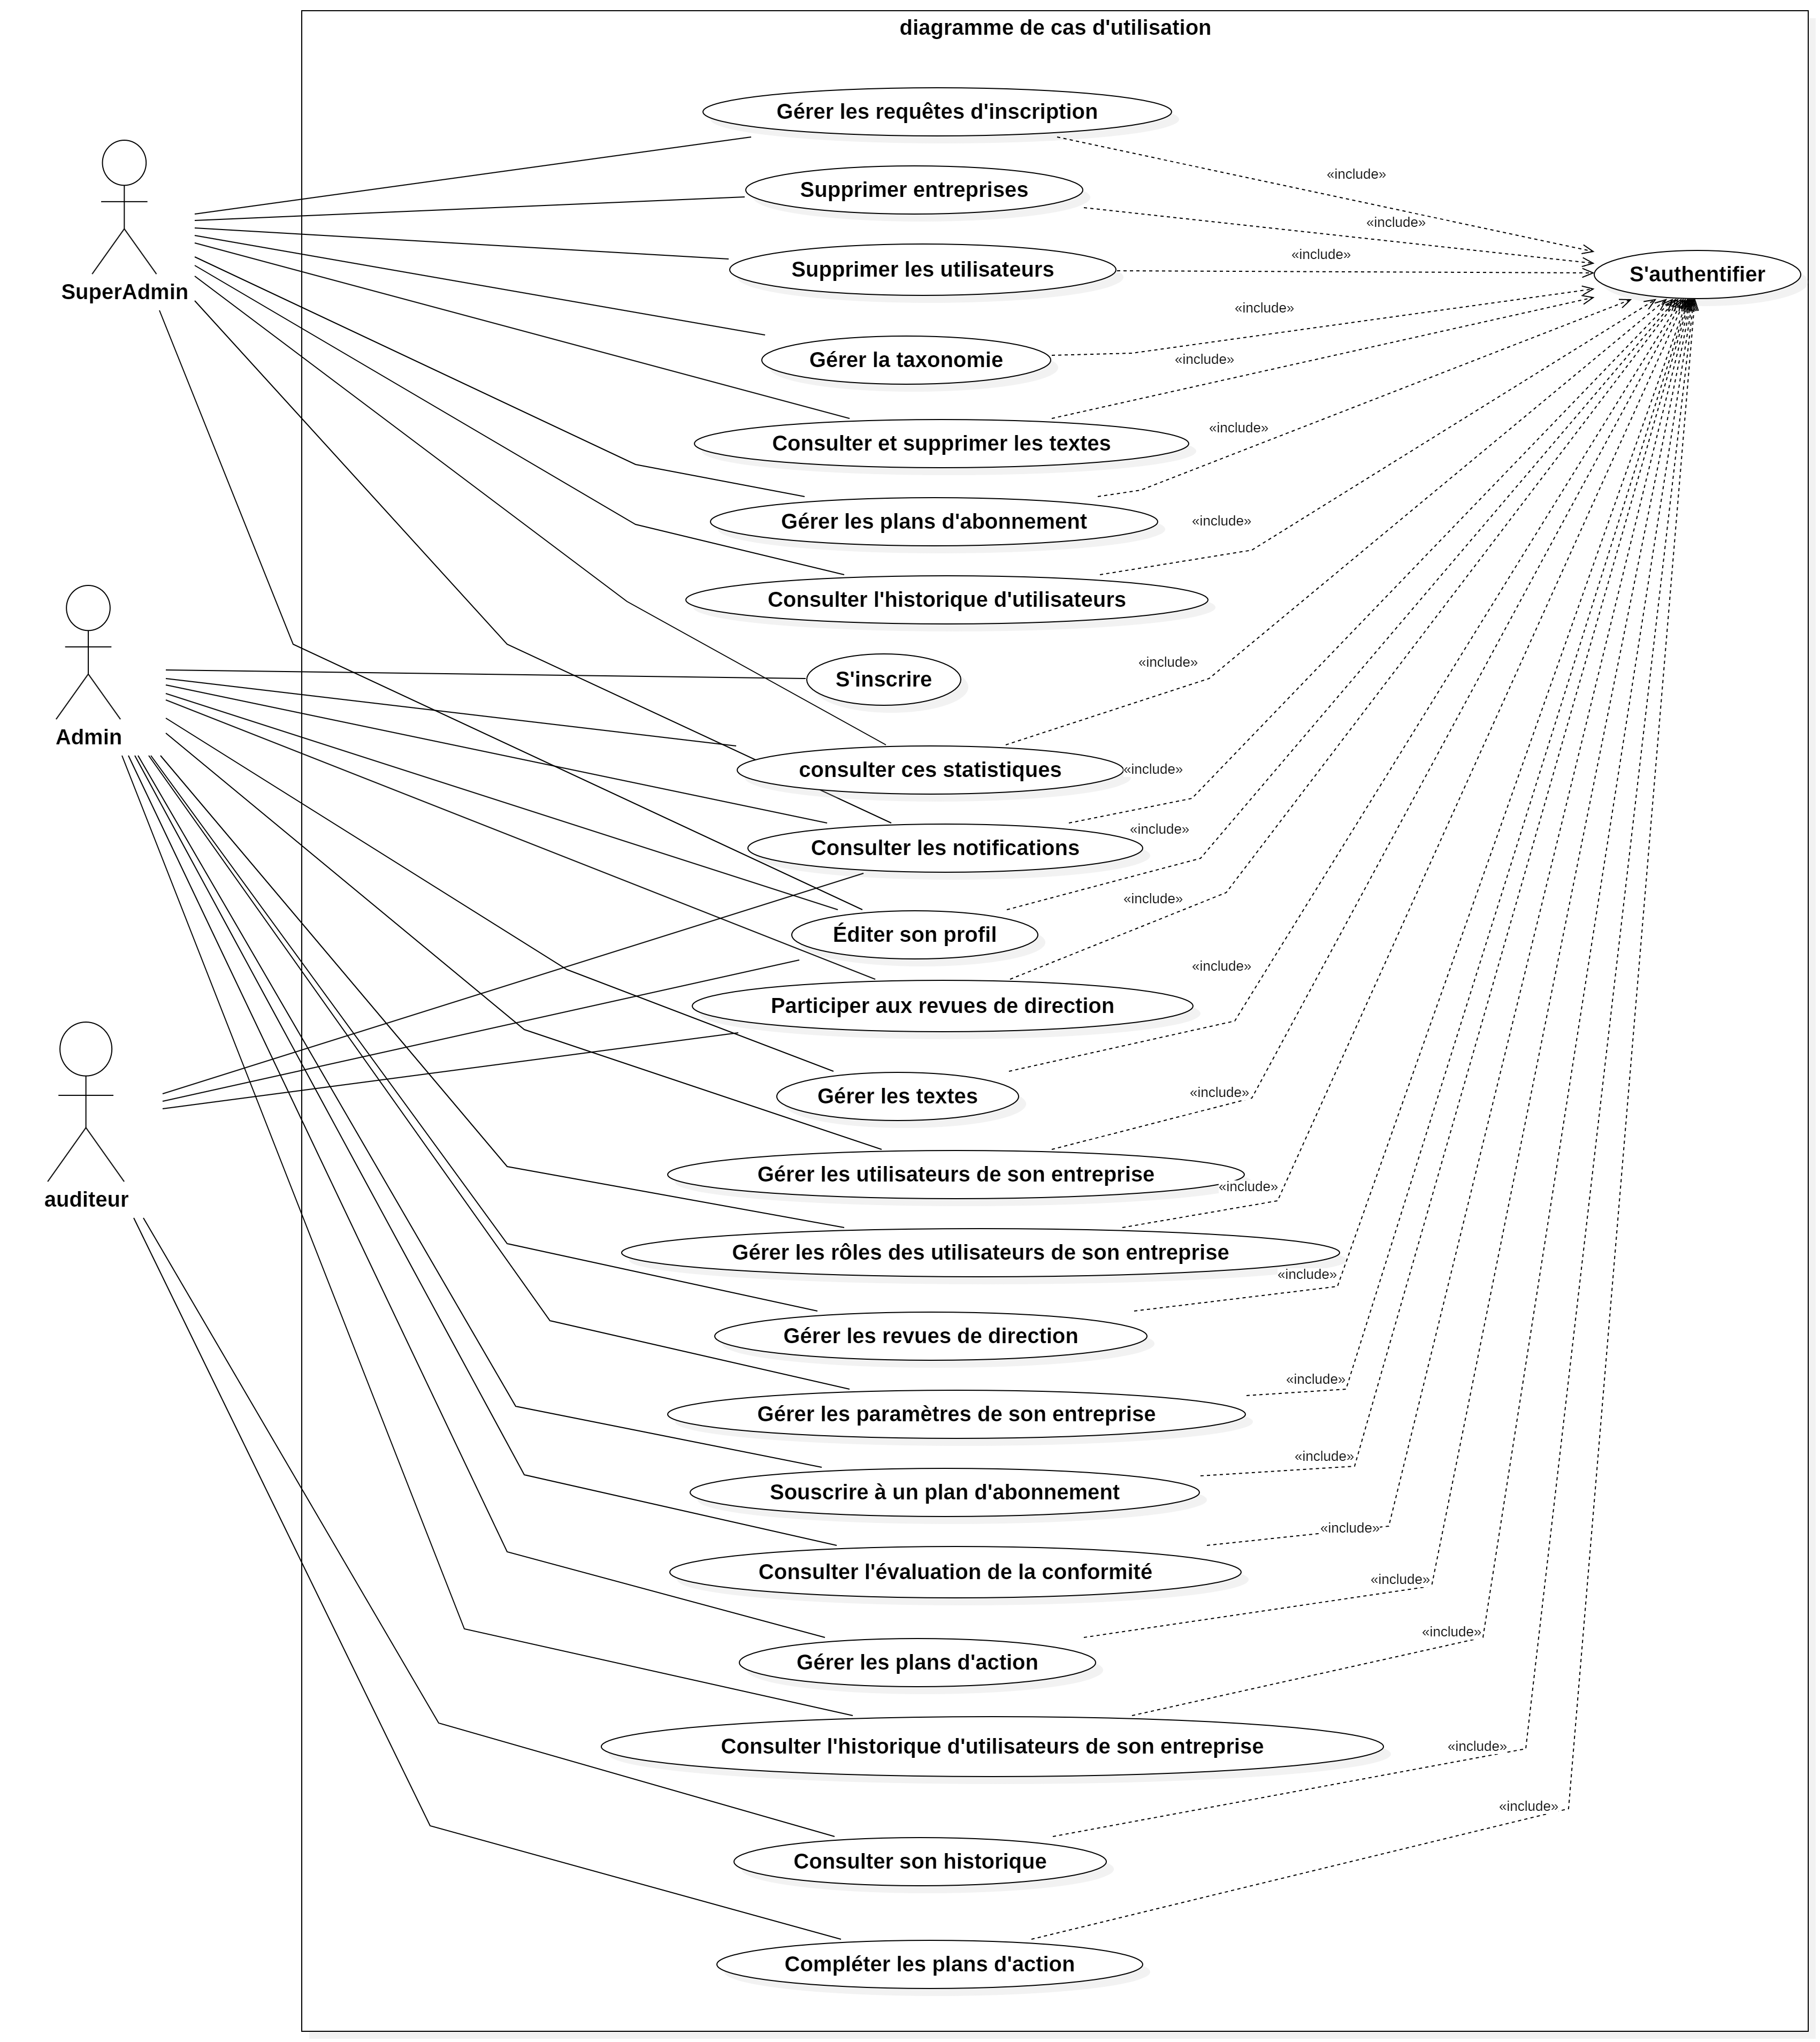
\includegraphics[width=18cm,height=20cm]{images/UseCaseDiagram.png}
    \caption{Diagramme de cas d'utilisation global}
\end{figure}

\subsection{Diagramme de classe globale :}

\noindent Le diagramme de classe globale en UML représente les objets du système, leurs attributs, leurs méthodes et leurs relations, décrivant l'architecture de l'application.

\begin{figure}[H]
    \centering
    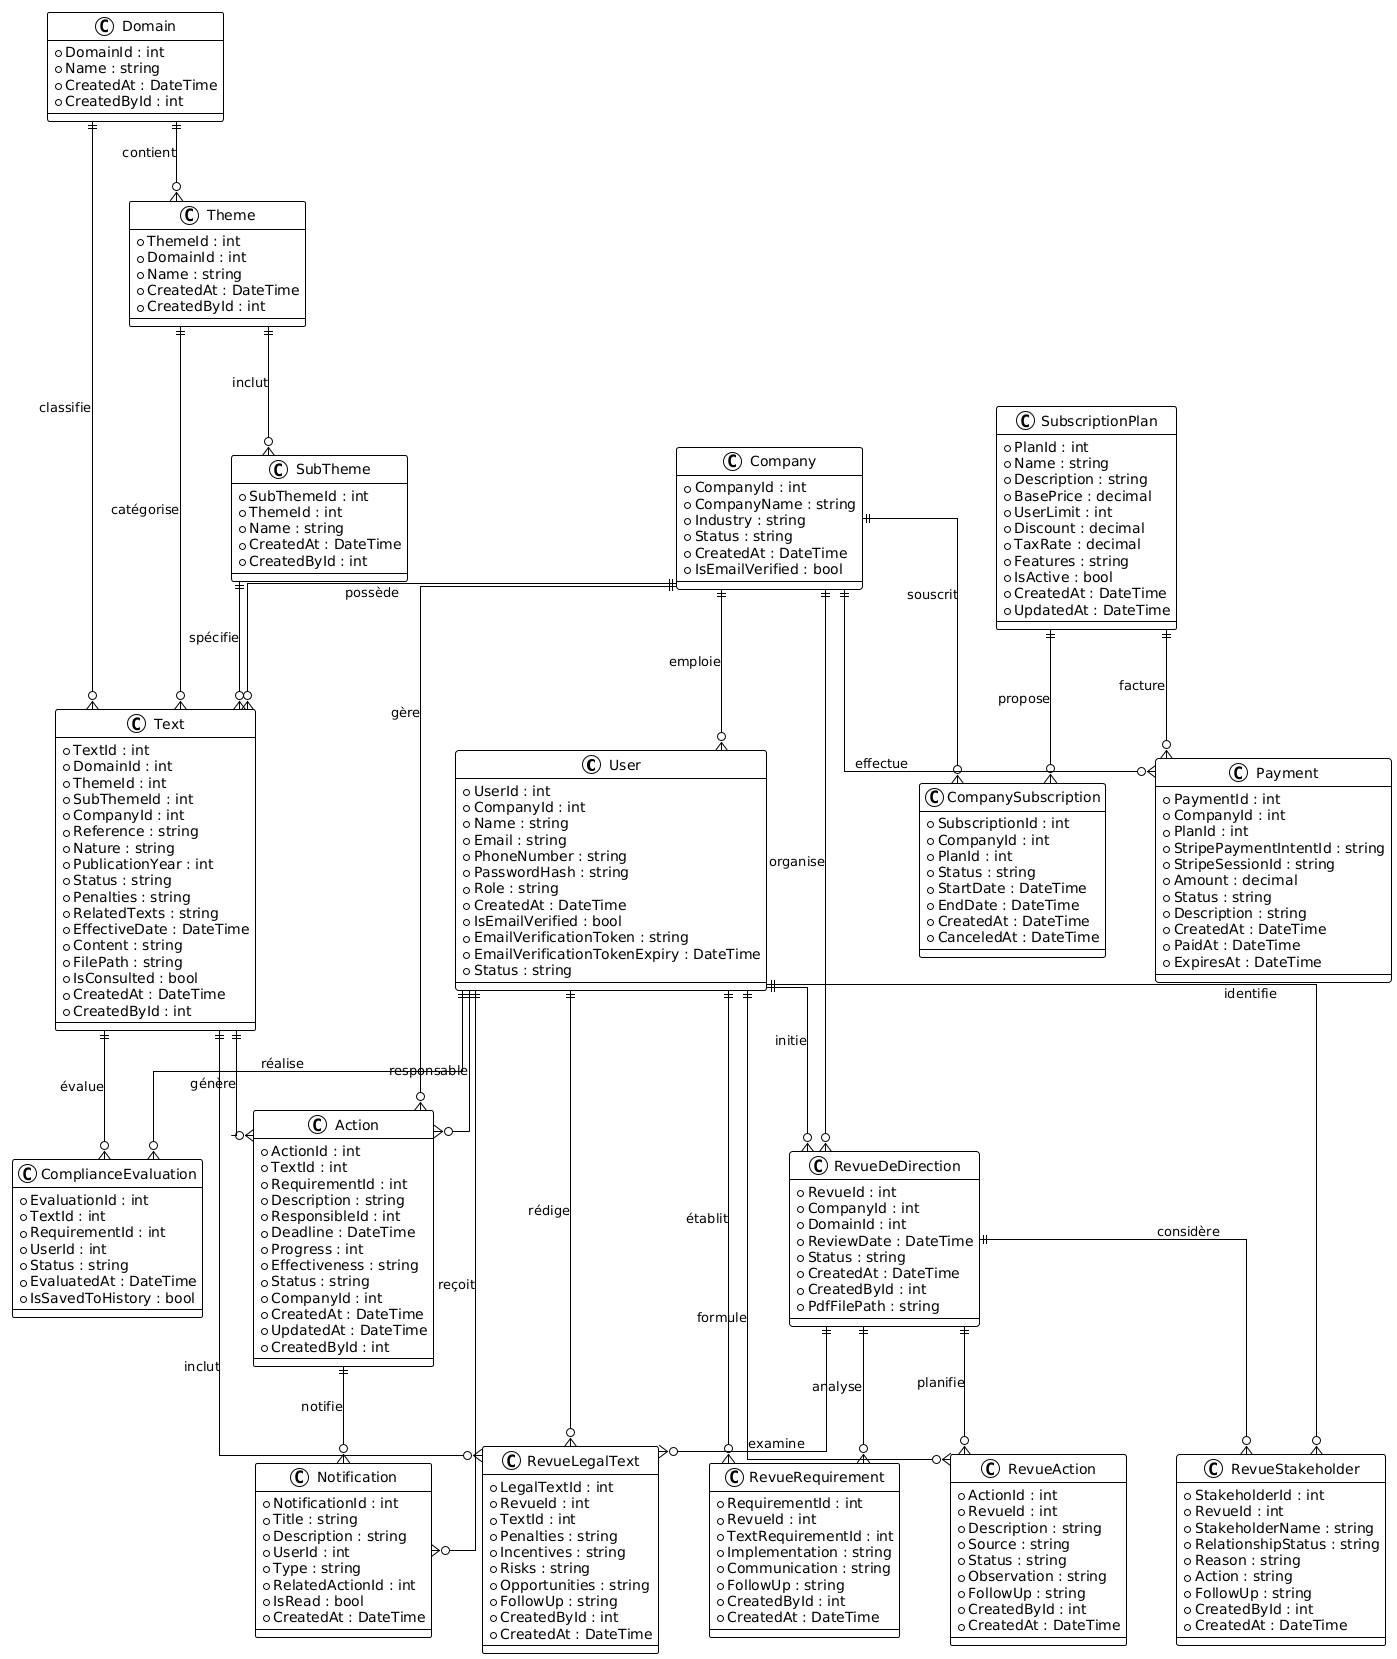
\includegraphics[width=18cm,height=19cm]{images/diagramclass.png}
    \caption{Diagramme des classes global}
\end{figure}

\section{Planifications des sprints :}

\noindent Le projet est structuré en quatre sprints répartis sur deux releases pour une livraison progressive et maîtrisée des fonctionnalités. Cette planification permet de prioriser les besoins essentiels tout en maintenant une approche itérative conforme à la méthodologie Scrum.

\begin{table}[h]
\centering
\caption{Planification des sprints}
\label{table:planification-sprints}
\begin{tabularx}{\textwidth}{|l|>{\raggedright\arraybackslash}X|>{\raggedright\arraybackslash}X|}
\hline
\textbf{Release} & \textbf{Sprint 1} & \textbf{Sprint 2} \\ \hline

\textbf{Release 1} &
\begin{minipage}[t]{\linewidth}
\vspace{2pt}
\textbf{Durée : 4 semaines}\\[0.4em]
• Authentification\\
• Inscription\\
• Gérer les requêtes d'inscription\\
• Gérer les profils
\vspace{2pt}
\end{minipage} &
\begin{minipage}[t]{\linewidth}
\vspace{2pt}
\textbf{Durée : 4 semaines}\\[0.4em]
• Gérer les utilisateurs\\
• Gérer les entreprises\\
• Gérer les paramètres d'entreprise\\
• Gérer la taxonomie
\vspace{2pt}
\end{minipage} \\ \hline

\textbf{Release 2} &
\begin{minipage}[t]{\linewidth}
\vspace{2pt}
\textbf{Durée : 6 semaines}\\[0.4em]
• Gérer les plans d'abonnement\\
• Souscrire aux abonnements\\
• Gérer les textes\\
• Consulter l'évaluation de conformité\\
• Gérer les plans d'action
\vspace{2pt}
\end{minipage} &
\begin{minipage}[t]{\linewidth}
\vspace{2pt}
\textbf{Durée : 6 semaines}\\[0.4em]
• Gérer les revues de direction\\
• Participer aux revues de direction\\
• Gérer les notifications\\
• Consulter l'historique\\
• Consulter les statistiques
\vspace{2pt}
\end{minipage} \\ \hline

\end{tabularx}
\end{table}


\section*{CONCLUSION}

\noindent Ce chapitre a permis de définir les acteurs, les besoins fonctionnels et non fonctionnels, ainsi que le backlog complet de l'application « Prévention Plus ». Les diagrammes UML et la planification des sprints ont clarifié l'organisation du développement. Le prochain chapitre abordera l'étude technique, détaillant les choix technologiques et la mise en œuvre.